\section{Capture and excitons}\label{sec:18.5}

A carrier in silicon whose kinetic energy has fallen below the impact-ionization threshold $\theta_{\mathrm{ii}}\Eg$ (\cref{sec:18.1}) can no longer add a pair. It reaches the band edge by emitting phonons within about a picosecond, and from then on the number of pairs $N_{\mathrm{eh}}$ whose mean and variance \cref{sec:18.2} computes is fixed. A detector at \SI{50}{mK} reads the event microseconds to seconds later. In that interval an electron can be captured by an ionized donor, or an electron and a hole can bind into an exciton. The exciton can bind to a neutral impurity, and the pair can recombine, giving its energy to the lattice or to a photon that leaves the crystal. Each of these processes changes what a charge or a heat readout records, and none of their rates has been measured at millikelvin temperatures in silicon or germanium. Without the rates one can still derive how each process changes the energy balance and the pair number.

\subsection{End-of-cascade capture}\label{sec:18.5-capture}

At the end of the cascade every carrier sits at a band edge, and the deposit is shared by the energy balance \cref{eq:18.1-energy}: $\Eg$ for each pair and the heat $E_{\mathrm{heat}}$ for the phonons emitted on the way down. This holds for an electron recoil, with no energy stored in defects and no photon leaving the crystal. Once carriers can be captured, not all of the energy outside the pairs is heat, and we name it separately,
\begin{equation}
  E_{\mathrm{np}} \equiv \omega - N_{\mathrm{eh}}\Eg ,
  \label{eq:18.5-Enp}
\end{equation}
the energy not held by pairs, equal to $E_{\mathrm{heat}}$ as long as nothing is captured. At fixed $\omega$ the pair number and $E_{\mathrm{np}}$ fluctuate together, $\operatorname{Var}N_{\mathrm{eh}} = \operatorname{Var}E_{\mathrm{np}}/\Eg^2$. From here on $N_{\mathrm{eh}}$ counts the electrons in the conduction band, free or bound to a hole in an exciton. An electron captured on an impurity level no longer counts.

Let an electron be captured on a level $E_j$ below the conduction-band edge $E_c$. The energy of a charge in the crystal is fixed relative to the Fermi level $\mu_F$ of the electrodes, since that is the energy the carrier gives up when it reaches one. A free electron holds $E_c - \mu_F$, a free hole $\mu_F - E_v$, with $E_v$ the valence-band edge, and a pair the sum, $\Eg$. After the capture the electron holds $E_j - \mu_F$, the phonons emitted at capture carry $E_c - E_j$, and the hole, now without a partner, still holds $\mu_F - E_v$. The three shares add to $\Eg$ whatever the level, and with $N_{\mathrm{eh}}$ lowered by one, \cref{eq:18.5-Enp} counts all three in $E_{\mathrm{np}}$; only the share $E_c - E_j$ is heat. A captured hole leaves $N_{\mathrm{eh}}$ unchanged; it changes the charge that the electrodes see, which is a matter of the readout.

Whether the electrons are captured is random. Let electron $i$ be captured with probability $f_i$, independently of the others once the cascade is given. The number of electrons left, $N'$, then has conditional mean $\sum_i(1 - f_i)$ and conditional variance $\sum_if_i(1 - f_i)$, a sum of Bernoulli variances. The law of total variance, $\operatorname{Var}N' = \langle\operatorname{Var}(N'|\text{cascade})\rangle + \operatorname{Var}\langle N'|\text{cascade}\rangle$, gives
\begin{equation}
  \langle N'\rangle = \Bigl\langle\sum_i(1 - f_i)\Bigr\rangle , \qquad
  \operatorname{Var}N' = \Bigl\langle\sum_if_i(1 - f_i)\Bigr\rangle + \operatorname{Var}\Bigl[\sum_i(1 - f_i)\Bigr] ,
  \label{eq:18.5-thingen}
\end{equation}
with the averages taken over cascades. If every electron has the same capture probability $f_{\mathrm{cap}}$, unrelated to the cascade, the sums become $(1 - f_{\mathrm{cap}})N_{\mathrm{eh}}$ and $f_{\mathrm{cap}}(1 - f_{\mathrm{cap}})N_{\mathrm{eh}}$, and the pair number is thinned binomially.

\begin{keyresult}[Capture at the end of the cascade]
Each electron captured before the readout raises the energy not held by pairs by exactly $\Eg$,
\begin{equation}
  E_{\mathrm{np}} \to E_{\mathrm{np}} + \Eg ,
  \label{eq:18.5-Eg}
\end{equation}
of which $E_c - E_j$ goes to phonons at the capture, $E_j - \mu_F$ stays with the trapped electron and $\mu_F - E_v$ with the unpaired hole. Let the capture probability $f_{\mathrm{cap}}$ be equal for all electrons and independent of the cascade. The mean energy per counted pair and the Fano factor of the counted pairs are then
\begin{equation}
  \varepsilon'_{\mathrm{eh}} = \frac{\varepsilon_{\mathrm{eh}}}{1 - f_{\mathrm{cap}}} , \qquad
  F'_{\mathrm{eh}} = (1 - f_{\mathrm{cap}})F_{\mathrm{eh}} + f_{\mathrm{cap}} .
  \label{eq:18.5-thin}
\end{equation}
A capture probability that depends on the carrier's state at the end of the cascade requires the general form \cref{eq:18.5-thingen}.
\end{keyresult}

The Fano factor of silicon is small, and \cref{eq:18.5-thin} makes it fragile: a loss raises it by $f_{\mathrm{cap}}(1 - F_{\mathrm{eh}})$, almost one for one. The cascade value 0.114 and the measured $0.119 \pm 0.002$ (\cref{sec:18.4}) differ by an amount that a loss of $f_{\mathrm{cap}} = \SI{0.54}{\percent}$ (0.32 to \SI{0.77}{\percent}) would produce, and the same loss raises $\varepsilon_{\mathrm{eh}}$ by \SI{0.55}{\percent}, which the calibration of the cascade on the measured pair energy absorbs. The Fano factor alone therefore cannot separate a sub-percent loss of pairs from the truncations of the cascade itself.

The binomial form fails when the capture probability depends on the energy $x_i$ that carrier $i$ still has after its last impact ionization. Those terminal energies are correlated with the pair number: \cref{sec:18.2} found that the residual energies of the terminal carriers anticorrelate with the phonon energy emitted above threshold. With $f_i = f(x_i)$ the variance term $\operatorname{Var}\sum_i(1 - f_i)$ is not, in general, $(1 - \bar f)^2\operatorname{Var}N_{\mathrm{eh}}$ with $\bar f$ the mean capture probability, and \cref{eq:18.5-thingen} has to be evaluated on the distribution of terminal energies that the cascade produces.

Capture is a collision of the kind that \cref{sec:18.1} turned into master-formula rates, with the potential of the impurity coupling the free carrier to a bound state and phonons carrying off the energy. Its size follows from a simpler argument. A carrier with kinetic energy $E$ is bound by an attractive center only if it comes within the distance at which the Coulomb energy equals its kinetic energy, $r_C(E) = \alpha/(\varepsilon_0E)$, and loses energy there. With $\hbar c$ restored, $\alpha = \SI{1.44}{eV.nm}$, and with the static constant of silicon at liquid-helium temperature, $\varepsilon_0 = 11.4$ (\cref{sec:7.4}), $\alpha/\varepsilon_0 = \SI{0.126}{eV.nm}$, so a carrier of \SI{0.1}{eV} has $r_C = \SI{1.26}{nm}$ and a capture cross-section of at most $\pi r_C^2 = \SI{5.0e-14}{cm^2}$; at \SI{0.35}{eV}, $r_C = \SI{0.36}{nm}$ and $\pi r_C^2 = \SI{4.1e-15}{cm^2}$. At a density of centers of \SI{e12}{cm^{-3}} the mean free path for capture is then at least \SI{20}{cm}, and it falls to micrometers only near \SI{e18}{cm^{-3}}. Capture of hot carriers during the cascade is negligible in a pure crystal. The cold carriers that the cascade leaves behind are a different matter. At the thermal energy of \SI{50}{mK}, $k_BT = \SI{4.3}{\micro eV}$, the Coulomb radius is $\alpha/(\varepsilon_0k_BT) = \SI{29}{\micro m}$, and a cold carrier finds any ionized center within tens of micrometers. The silicon detectors of CDMS~II, the second phase of the Cryogenic Dark Matter Search (CDMS), for example, were operated with their ionized trapping sites neutralized by regular exposure to infrared light-emitting diodes, which left the bulk in a metastable state with low trapping~\cite[Sect.~2]{agnese2018nuclear}. Capture on neutral centers and capture during drift belong to the readout, and every one of them adds the same $\Eg$ to $E_{\mathrm{np}}$.

\begin{workedexample}{One captured electron in ten pairs}\label{we:18-capture}
An electron recoil of $\omega = \SI{37.5}{eV}$ in silicon makes about ten pairs at the measured $\varepsilon_{\mathrm{eh}} = \SI{3.75}{eV}$ of \cref{sec:1.5}. Take an event with exactly ten. With $\Eg = \SI{1.17}{eV}$, the energy balance gives $E_{\mathrm{heat}} = E_{\mathrm{np}} = 37.5 - 10\times1.17 = \SI{25.80}{eV}$ in phonons. Let one electron be captured by an ionized phosphorus donor, whose ground state lies \SI{45.6}{meV} below the band edge (\cref{sec:7.4}). The pair number falls to nine and $E_{\mathrm{np}} = 37.5 - 9\times1.17 = \SI{26.97}{eV}$, larger by exactly $\Eg$. Of that \SI{1.17}{eV}, \SI{45.6}{meV} is emitted as phonons when the electron drops onto the donor, and \SI{1.124}{eV} stays as the potential energy of the trapped electron and of its unpaired hole, divided between them according to where $\mu_F$ lies. A charge readout calibrated at \SI{3.75}{eV} per pair reports $9\times3.75 = \SI{33.75}{eV}$; the energy per counted pair of this event is $37.5/9 = \SI{4.17}{eV}$, \SI{11.1}{\percent} above $\varepsilon_{\mathrm{eh}}$.

Now let each of the electrons be captured with probability $f_{\mathrm{cap}} = 0.1$ instead. The mean number counted is nine, the same as before, and $\varepsilon'_{\mathrm{eh}} = 3.75/0.9 = \SI{4.17}{eV}$ by \cref{eq:18.5-thin}. With the measured $F_{\mathrm{eh}} = 0.119$, however, the Fano factor rises to $F'_{\mathrm{eh}} = 0.9\times0.119 + 0.1 = 0.207$, and the standard deviation of the counted pairs from $(0.119\times10)^{1/2} = 1.09$ to $(0.207\times9)^{1/2} = 1.37$. A capture of fixed size shifts the yield; a capture at random also broadens it. Of the variance $0.207\times9 = 1.86$, the thinned cascade contributes $0.9^2\times1.19 = 0.96$ and the binomial choice of which electrons are captured $0.1\times0.9\times10 = 0.90$, almost as much.
\end{workedexample}

\subsection{Excitons and the measured Fano factor}\label{sec:18.5-excitons}

A cold electron and hole left near each other at zero field bind. The binding energy of the silicon exciton, $E_x^b = \SI{14.7}{meV}$ (\cref{sec:4.9}), is 3400 times $k_BT$ at \SI{50}{mK}, and a pair closer than the \SI{29}{\micro m} Coulomb radius found above cannot be pulled apart by thermal motion. Binding is a two-body process that waits for both carriers to cool by emitting acoustic phonons, slow at millikelvin temperatures, so it takes place after the cascade has fixed $N_{\mathrm{eh}}$. Since $N_{\mathrm{eh}}$ counts bound pairs, an exciton changes neither $N_{\mathrm{eh}}$ nor $\varepsilon_{\mathrm{eh}}$ nor $F_{\mathrm{eh}}$. What it changes is where the energy sits: a bound pair holds $\Eg - E_x^b$, and the binding energy goes to the lattice.

A heat readout, however, sees more than $E_{\mathrm{np}}$. With $N_X$ bound pairs at readout and no capture, the phonon energy is $E_{\mathrm{heat}} = E_{\mathrm{np}} + N_XE_x^b$. Its mean rises by $E_x^b$ per bound pair, at most $E_x^b/\varepsilon_{\mathrm{eh}} = \SI{0.39}{\percent}$ of $\omega$ in silicon. Define the Fano factor inferred from the phonon energy, $F_{\mathrm{heat}} \equiv \operatorname{Var}E_{\mathrm{heat}}/(\Eg^2\langle N_{\mathrm{eh}}\rangle)$. It differs from $F_{\mathrm{eh}} = \operatorname{Var}E_{\mathrm{np}}/(\Eg^2\langle N_{\mathrm{eh}}\rangle)$ by the variance of $N_X$ and its covariance with $E_{\mathrm{np}}$,
\begin{equation}
  F_{\mathrm{heat}} = F_{\mathrm{eh}} + \frac{(E_x^b)^2\operatorname{Var}N_X + 2E_x^b\operatorname{Cov}(E_{\mathrm{np}}, N_X)}{\Eg^2\langle N_{\mathrm{eh}}\rangle} .
  \label{eq:18.5-Fheat}
\end{equation}
When every pair binds, $N_X = N_{\mathrm{eh}}$ and $E_{\mathrm{heat}} = \omega - N_{\mathrm{eh}}(\Eg - E_x^b)$, so $F_{\mathrm{heat}} = F_{\mathrm{eh}}(1 - E_x^b/\Eg)^2$: \SI{2.5}{\percent} below $F_{\mathrm{eh}}$ in silicon, and 0.7 to \SI{1.3}{\percent} in germanium, whose indirect exciton is bound by a few meV, 2.5 and \SI{5}{meV} in absorption~\cite{zwerdling1959exciton,macfarlane1957fine}, against a gap of \SI{0.744}{eV}.

A charge readout is affected only if the exciton is never split. A bound pair is neutral and drifts as a whole, so it induces no charge on the electrodes. Let each pair independently end as such an exciton with probability $p_{\mathrm{ns}}$. The counted charge is then thinned exactly as by capture, and by the algebra of \cref{eq:18.5-thin} its Fano factor is
\begin{equation}
  F_{\mathrm{meas}} = (1 - p_{\mathrm{ns}})F_{\mathrm{eh}} + p_{\mathrm{ns}} ,
  \label{eq:18.5-Fmeas}
\end{equation}
where $F_{\mathrm{meas}}$ is the Fano factor of the measured charge, before the corrections of the readout itself. A heat readout thus sees $F_{\mathrm{heat}}$ and a charge readout $F_{\mathrm{meas}}$, while $F_{\mathrm{eh}}$, which counts bound and free pairs alike, is the cascade value that neither changes. In a biased detector the field can separate the pair before it binds. The force $e\mathcal{E}$ of a field $\mathcal{E}$ exceeds the attraction $\alpha/(\varepsilon_0r^2)$ beyond the radius
\begin{equation}
  r_{\mathcal{E}} = \Bigl(\frac{\alpha}{\varepsilon_0e\mathcal{E}}\Bigr)^{1/2} ,
  \label{eq:18.5-rfield}
\end{equation}
which in silicon is \SI{0.56}{\micro m} at \SI{4}{V/cm} and \SI{0.11}{\micro m} at \SI{100}{V/cm}. A pair that ends the cascade farther apart than $r_{\mathcal{E}}$ is separated; a closer one can bind, and once bound it stays bound, since the field that ionizes the exciton is of order $E_x^b/(ea_x) = \SI{3.5e4}{V/cm}$, with $a_x = \SI{4.2}{nm}$ (\cref{sec:4.9}). Exciton formation thus changes the measured Fano factor through \cref{eq:18.5-Fmeas} when the readout field is weak enough that $r_{\mathcal{E}}$ exceeds the separation of the pairs at the end of the cascade, a distribution the cascade calculation has to supply. When excitons form from carriers of different pairs, as in a dense track, the loss is not independent from pair to pair, its probability grows with the density, and the variance acquires a part that grows faster than $\langle N_{\mathrm{eh}}\rangle$.

One process acts on the cascade itself. A carrier with energy between $\Eg - E_x^b$ and the ionization threshold can create a bound pair directly, which acts for that pair like a gap lowered by $E_x^b$. With the slope $\partial\varepsilon_{\mathrm{eh}}/\partial\Eg = 1.70$ of the calibrated cascade at fixed $A_{\mathrm{AB}}$ (\cref{sec:18.4-three}), the pair energy moves by at most $1.70E_x^b = \SI{25}{meV}$ in silicon, \SI{0.67}{\percent}, and \SI{8.6}{meV} in germanium, \SI{0.30}{\percent}, for the larger of its two measured binding energies. In ionic crystals with excitons bound by about \SI{1}{eV}, the bound pair and not the free pair may be the unit the cascade produces, and the excitons self-trap (\cref{sec:10.5}); their pair energies lie outside the range in which the cascade model was validated (\cref{sec:18.4}).

\subsection{Rate equations at millikelvin}\label{sec:18.5-kinetics}

After the cascade each pair is in one of four kinds of state: a free pair $F$, a free exciton $X$, an exciton $B_j$ bound to a neutral impurity of species $j$, or a pair with a carrier trapped on a center of species $j$. In the dilute clouds of electron recoils each pair evolves on its own, with its own partner or with a fixed background center. Every transition is then first order in the occupation of the pair's own state. For the occupation probabilities $p_F$, $p_X$ and $p_{B,j}$ of one pair,
\begin{equation}
  \begin{aligned}
    \frac{\dd p_F}{\dd t} &= -(\varGamma_{FX} + \varGamma_{FT})\,p_F , \\
    \frac{\dd p_X}{\dd t} &= \varGamma_{FX}\,p_F - \Bigl(\varGamma_X + \sum_j\varGamma_{XB,j}\Bigr)p_X , \\
    \frac{\dd p_{B,j}}{\dd t} &= \varGamma_{XB,j}\,p_X - \varGamma_{B,j}\,p_{B,j} .
  \end{aligned}
  \label{eq:18.5-rates}
\end{equation}
Here $\varGamma_{FX}$ is the rate at which the pair binds and $\varGamma_{FT}$ the rate at which one of its carriers is trapped. The free exciton decays at the rate $\varGamma_X$, a fraction $\eta_X$ of it by luminescence, and binds to impurities of density $\nd_j$ at the rate $\varGamma_{XB,j} = \sigma_{XB,j}v_X\nd_j$, with cross-section $\sigma_{XB,j}$ and exciton speed $v_X$. The bound exciton decays at the rate $\varGamma_{B,j}$, a fraction $\eta_{B,j}$ of it by luminescence. In silicon a bound exciton decays mostly by an Auger process: the pair recombines and gives its energy to the extra carrier of the complex, which is ejected and leaves the impurity ionized. Its lifetime at the phosphorus donor is 200 to \SI{300}{ns} at liquid-helium temperature, as quoted by Lo and coworkers~\cite{lo2015hybrid}. No reverse steps appear: dissociating an exciton or freeing it from an impurity costs $E_x^b$ or more, thousands of times $k_BT$ at \SI{50}{mK}.

The trapped carriers follow the occupation $\nd^{\mathrm{tr}}_j$ of each species of center,
\begin{equation}
  \frac{\dd\nd^{\mathrm{tr}}_j}{\dd t} = \sigma_{\mathrm{cap},j}u\,\nd_{\mathrm{c}}\bigl(\nd_j - \nd^{\mathrm{tr}}_j\bigr) - \varGamma^{\mathrm{em}}_j\nd^{\mathrm{tr}}_j - \sigma^{\mathrm{rec}}_ju\,\nd_{\mathrm{v}}\nd^{\mathrm{tr}}_j ,
  \label{eq:18.5-traps}
\end{equation}
written for electrons, with free-electron and free-hole densities $\nd_{\mathrm{c}}$ and $\nd_{\mathrm{v}}$ and carrier speed $u$. The center captures with the cross-section $\sigma_{\mathrm{cap},j}$, emits at the rate $\varGamma^{\mathrm{em}}_j$, and loses its electron to a free hole with the cross-section $\sigma^{\mathrm{rec}}_j$; holes obey the same equation with the roles exchanged. Thermal emission is frozen. For the phosphorus donor the Boltzmann exponent at \SI{50}{mK} is $(\SI{45.6}{meV})/k_BT = 1.06\times10^4$. A field lowers the barrier of a Coulomb center: the potential $-\alpha/(\varepsilon_0r) - e\mathcal{E}r$ along the field has its maximum at $r_{\mathcal{E}}$ of \cref{eq:18.5-rfield}, lower than the zero-field barrier by $2(\alpha e\mathcal{E}/\varepsilon_0)^{1/2}$, the Poole--Frenkel lowering. At \SI{100}{V/cm} it is \SI{2.25}{meV}, and the exponent stays at $1.0\times10^4$. A trapped carrier is released only athermally, by the phonons and hot carriers of later events or by infrared light, so the occupations carry the history of earlier events into later ones, the source of delayed charge (\cref{app:E.25}).

Without reverse steps the matrix of \cref{eq:18.5-rates} is lower triangular in the order $F$, $X$, $B_j$, and its decay constants $\gamma_k$ are its diagonal entries, $\varGamma_{FX} + \varGamma_{FT}$, $\varGamma_X + \sum_j\varGamma_{XB,j}$ and $\varGamma_{B,j}$. The fraction of the gap energy still held by pairs and excitons,
\begin{equation}
  r_{\mathrm{gap}}(t) = p_F + p_X + \sum_jp_{B,j} = \sum_kw_k\,\ee^{-\gamma_kt} , \qquad \sum_kw_k = 1 ,
  \label{eq:18.5-rgap}
\end{equation}
decays as a sum of exponentials when the $\gamma_k$ are distinct, up to the binding energies. An exciton bound to a phosphorus donor sits a further \SI{5}{meV} or so below the free exciton~\cite{lo2015hybrid}, so $r_{\mathrm{gap}}$ overstates the held energy by at most $(E_x^b + \SI{5}{meV})/\Eg = \SI{1.7}{\percent}$ in silicon. The weights $w_k$ need not be positive: a transfer from $X$ to $B_j$ without loss delays the decay, and its weight is negative. To see where the gap energy ends up, we integrate the occupations over time, $\int_0^\infty p\,\dd t = -M^{-1}p(0)$ for the matrix $M$ of \cref{eq:18.5-rates} and a pair that starts free. They are $\int p_F = 1/(\varGamma_{FX} + \varGamma_{FT})$, $\int p_X = \varGamma_{FX}\int p_F/(\varGamma_X + \sum_j\varGamma_{XB,j})$ and $\int p_{B,j} = \varGamma_{XB,j}\int p_X/\varGamma_{B,j}$, and multiplying each by its outgoing rates gives
\begin{equation}
  b_{\mathrm{trap}} = \frac{\varGamma_{FT}}{\varGamma_{FX} + \varGamma_{FT}} , \qquad
  b_{\mathrm{light}} = (1 - b_{\mathrm{trap}})\,\frac{\varGamma_X\eta_X + \sum_j\varGamma_{XB,j}\eta_{B,j}}{\varGamma_X + \sum_j\varGamma_{XB,j}} , \qquad
  b_{\mathrm{heat}} = 1 - b_{\mathrm{trap}} - b_{\mathrm{light}}
  \label{eq:18.5-split}
\end{equation}
for the fractions of the gap energy that end trapped, as escaping light and as phonons. The trapped and escaping fractions are lost to a heat readout at any window, while the phonon fraction arrives only as fast as $r_{\mathrm{gap}}$ decays.

\Cref{fig:18-end} shows the populations of a pair in silicon at \SI{50}{mK} for one set of rates. The bound-exciton decay uses the measured Auger lifetime; the other rates are chosen only to show how the solution behaves. The pair binds within a nanosecond, the bound-exciton population peaks at 0.15 near \SI{0.45}{\micro s}, half of the gap energy is still held by pairs and excitons at \SI{0.83}{\micro s}, when phonons carry 0.445 of it, and \SI{1}{\percent} at \SI{4.4}{\micro s}. The weights of $r_{\mathrm{gap}}$ are $+1.28$ for the free exciton, $-0.33$ for the bound one and $+0.05$ for the free pair. A heat readout that closes its window at \SI{1}{\micro s} misses the \SI{42}{\percent} of the gap energy still held in this model, plus the \SI{5.6}{\percent} already trapped or radiated, and the window dependence enters the heat yield of any phonon readout. In the dense tracks of nuclear recoils the pairs are not independent, and two-body processes take over. Binding of carriers from different pairs moves gap energy from pairs to excitons and leaves $r_{\mathrm{gap}}$ unchanged; exciton--exciton annihilation and Auger recombination of free carriers remove it, and they make $r_{\mathrm{gap}}$ fall as a power of time at a rate set by the track density. Since that density differs between nuclear and electron recoils of the same energy, so does $r_{\mathrm{gap}}$ at a given window.

\begin{figure}[tbp]
  \centering
  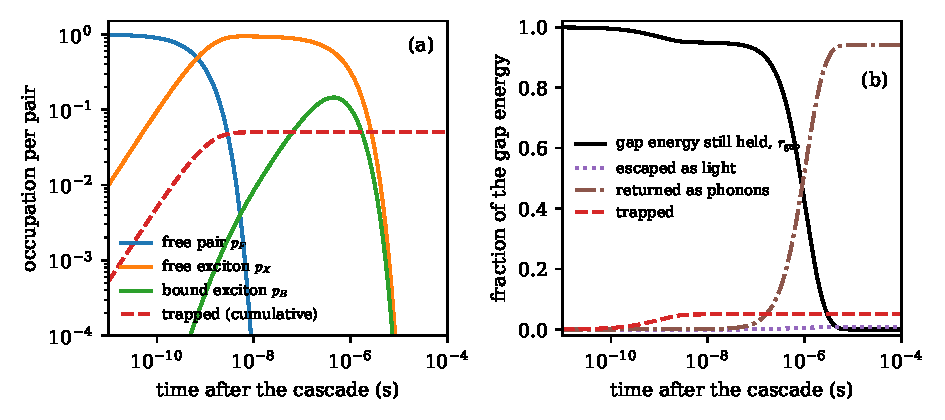
\includegraphics[width=\linewidth]{figures/ch18/fig18_4.pdf}
  \caption{End-of-cascade populations of one electron--hole pair in silicon at \SI{50}{mK}, from the rate equations \cref{eq:18.5-rates} with one species of neutral impurity. (a)~Occupations of the free pair, the free exciton and the bound exciton, and the cumulative trapped fraction, against the time after the cascade. (b)~Fraction of the gap energy still held by pairs and excitons, $r_{\mathrm{gap}}$ of \cref{eq:18.5-rgap}, and the cumulative fractions returned as phonons, escaped as light and trapped. Rates: bound-exciton Auger decay \SI{250}{ns}, inside the measured 200 to \SI{300}{ns} of the phosphorus donor~\cite{lo2015hybrid}, without light. Illustrative, since none is measured at \SI{50}{mK}: binding of the pair \SI{1}{ns}, trapping $\varGamma_{FT} = 0.053\varGamma_{FX}$, binding of the free exciton to impurities \SI{1}{\micro s}, free-exciton decay \SI{10}{\micro s} with luminescent fraction 0.1. Asymptotic split \cref{eq:18.5-split}: 0.050 trapped, 0.009 light, 0.941 phonons.}
  \label{fig:18-end}
\end{figure}

\subsection{Unknown rates and unsized truncations}\label{sec:18.5-open}

The rates of \cref{eq:18.5-rates,eq:18.5-traps} are the main unknowns of this section. In silicon and germanium at 10 to \SI{50}{mK}, no measurement or calculation gives the rate at which a cold pair binds, or the coefficient of binding between carriers of different pairs. The same holds for the capture cross-sections of cold and drifting carriers on charged and neutral centers, as functions of carrier energy, temperature and field, and for the cross-sections for binding of excitons to each impurity species. Also unknown are the decay rate and luminescent fraction of the free exciton, the luminescent fractions of the bound excitons, and the coefficients of exciton--exciton annihilation and of Auger recombination that govern dense tracks. The thresholds at which dense pairs condense into electron--hole droplets, the degenerate electron--hole liquid of germanium and silicon, are open as well at millikelvin temperatures. What is known are the binding energies, \SI{14.7}{meV} in silicon and a few meV in germanium, and the Auger lifetimes of bound excitons at liquid-helium temperature, a property of the complex in its ground state that should carry over to lower temperatures. The excitons themselves cool by emitting acoustic phonons, slowly at these temperatures, so their temperature need not be that of the lattice, and rates measured at a few kelvin cannot simply be transferred.

The cascade hands over less than these equations need. No material has a computed capture probability $f(x)$ as a function of the terminal energy of a carrier, nor the distribution of terminal energies on which \cref{eq:18.5-thingen} averages it. Nor is the separation of the pairs at the end of the cascade, which decides through \cref{eq:18.5-rfield} whether a field prevents binding. In the ionic crystals, where the cascade quantum may be a bound pair, the exciton binding energies and the binding to impurities are open as well.

Two approximations of the cascade itself remain unsized. A constant factor of 0.8 on the impact-ionization rate, the quasiparticle residue left out of \cref{eq:18.1-ii}, changes $\varepsilon_{\mathrm{eh}}$ by about \SI{3}{\percent}, and calibrating on the measured pair energy removes it. A factor that varies with the carrier energy between threshold and about \SI{10}{eV}, as the residue and the carrier--electron exchange may, changes $F_{\mathrm{eh}}$, and its size is not known. For the energy-only reduction, the probability that a carrier keeps its momentum between two events that change its energy is estimated to be below about 0.1 within \SI{1}{eV} of threshold, where intervalley scattering dominates, and to reach one half above 3 to \SI{5}{eV} in silicon. A full-band cascade finds the resulting memory negligible, but only within the deformation-potential model of the phonons (\cref{sec:18.1-reductions}); with first-principles couplings, which do not redraw the crystal momentum at every emission, neither this probability nor the spread over the iso-energy surface that it multiplies has been computed.
